% Options for packages loaded elsewhere
\PassOptionsToPackage{unicode}{hyperref}
\PassOptionsToPackage{hyphens}{url}
\PassOptionsToPackage{dvipsnames,svgnames,x11names}{xcolor}
%
\documentclass[
  13pt,
  ignorenonframetext,
]{beamer}
\usepackage{pgfpages}
\setbeamertemplate{caption}[numbered]
\setbeamertemplate{caption label separator}{: }
\setbeamercolor{caption name}{fg=normal text.fg}
\beamertemplatenavigationsymbolsempty
% Prevent slide breaks in the middle of a paragraph
\widowpenalties 1 10000
\raggedbottom
\setbeamertemplate{part page}{
  \centering
  \begin{beamercolorbox}[sep=16pt,center]{part title}
    \usebeamerfont{part title}\insertpart\par
  \end{beamercolorbox}
}
\setbeamertemplate{section page}{
  \centering
  \begin{beamercolorbox}[sep=12pt,center]{part title}
    \usebeamerfont{section title}\insertsection\par
  \end{beamercolorbox}
}
\setbeamertemplate{subsection page}{
  \centering
  \begin{beamercolorbox}[sep=8pt,center]{part title}
    \usebeamerfont{subsection title}\insertsubsection\par
  \end{beamercolorbox}
}
\AtBeginPart{
  \frame{\partpage}
}
\AtBeginSection{
  \ifbibliography
  \else
    \frame{\sectionpage}
  \fi
}
\AtBeginSubsection{
  \frame{\subsectionpage}
}

\usepackage{amsmath,amssymb}
\usepackage{iftex}
\ifPDFTeX
  \usepackage[T1]{fontenc}
  \usepackage[utf8]{inputenc}
  \usepackage{textcomp} % provide euro and other symbols
\else % if luatex or xetex
  \usepackage{unicode-math}
  \defaultfontfeatures{Scale=MatchLowercase}
  \defaultfontfeatures[\rmfamily]{Ligatures=TeX,Scale=1}
\fi
\usepackage{lmodern}
\ifPDFTeX\else  
    % xetex/luatex font selection
\fi
% Use upquote if available, for straight quotes in verbatim environments
\IfFileExists{upquote.sty}{\usepackage{upquote}}{}
\IfFileExists{microtype.sty}{% use microtype if available
  \usepackage[]{microtype}
  \UseMicrotypeSet[protrusion]{basicmath} % disable protrusion for tt fonts
}{}
\makeatletter
\@ifundefined{KOMAClassName}{% if non-KOMA class
  \IfFileExists{parskip.sty}{%
    \usepackage{parskip}
  }{% else
    \setlength{\parindent}{0pt}
    \setlength{\parskip}{6pt plus 2pt minus 1pt}}
}{% if KOMA class
  \KOMAoptions{parskip=half}}
\makeatother
\usepackage{xcolor}
\newif\ifbibliography
\setlength{\emergencystretch}{3em} % prevent overfull lines
\setcounter{secnumdepth}{-\maxdimen} % remove section numbering


\providecommand{\tightlist}{%
  \setlength{\itemsep}{0pt}\setlength{\parskip}{0pt}}\usepackage{longtable,booktabs,array}
\usepackage{calc} % for calculating minipage widths
\usepackage{caption}
% Make caption package work with longtable
\makeatletter
\def\fnum@table{\tablename~\thetable}
\makeatother
\usepackage{graphicx}
\makeatletter
\def\maxwidth{\ifdim\Gin@nat@width>\linewidth\linewidth\else\Gin@nat@width\fi}
\def\maxheight{\ifdim\Gin@nat@height>\textheight\textheight\else\Gin@nat@height\fi}
\makeatother
% Scale images if necessary, so that they will not overflow the page
% margins by default, and it is still possible to overwrite the defaults
% using explicit options in \includegraphics[width, height, ...]{}
\setkeys{Gin}{width=\maxwidth,height=\maxheight,keepaspectratio}
% Set default figure placement to htbp
\makeatletter
\def\fps@figure{htbp}
\makeatother

%\ProvidesPackage{config/presento}

\mode<presentation>

% removing navigation symbols
\setbeamertemplate{navigation symbols}{}

% packages
\usepackage{xcolor}
\usepackage{fontspec}
\usepackage{setspace}
\usepackage{tikz}
\usepackage{soul}
\usepackage{multicol}
\usepackage{multirow}
\usepackage{philex}

% colors
\definecolor{colorblack}{HTML}{000000} % for note
\definecolor{colorgreen}{HTML}{009933} % for code
\definecolor{colorwhite}{HTML}{FFFFFF} % background
\definecolor{colorblue}{HTML}{0099CC} % blue
\definecolor{colorbig}{HTML}{1f77b4} % for note
\definecolor{colormedium}{HTML}{ff7f0e} % for note
\definecolor{colorsmall}{HTML}{2ca02c} % for note


% font sizes
\newcommand{\fontsizeone}{1em}
\newcommand{\fontsizetwo}{0.85em}
\newcommand{\fontsizethree}{1em}
% line spaces
\newcommand{\linespaceone}{1}

% font families
\newfontfamily{\inconsolatafont}[Path=fonts/]{brill}

% beamer template changes
\setbeamertemplate{frametitle}{
 \vspace{0.40em}
 \noindent
 \hspace{-1.22em}
 \tikz[overlay,remember picture,baseline=0.3em]{\fill[fill= colorblue]  (-0.3,0.05) rectangle (0,0.9); }\color{colorblue}~~\insertframetitle%
}

\setmainfont[Ligatures=TeX,Path=fonts/,
						BoldFont=brillb,
						ItalicFont=brilli,
						BoldItalicFont=brillbi,
						SmallCapsFont=brill]{brill}
\setsansfont[Ligatures=TeX,Path=fonts/,
						BoldFont=brillb,
						ItalicFont=brilli,
						BoldItalicFont=brillbi,
						SmallCapsFont=brill]{brill}
\setmonofont[Scale=0.7, Path=fonts/]{iosevka-regular}

% frame counter
\newcounter{totalfr}
\setbeamertemplate{footline}{
  \ifnum\inserttotalframenumber=1
    \setcounter{totalfr}{2}
  \else
     \setcounter{totalfr}{\inserttotalframenumber}
  \fi
  \hfill{
    \tikz{
      \filldraw[fill=colorblue!80, draw=colorblue!80]  (0,0) -- (0.2,0) arc (0:{\value{framenumber}*(360/(\value{totalfr}))}:0.2) -- (0,0); 
      \node at (0,0) {\normalsize \color{colorblack}\tiny{\insertframenumber}};
    }
  }
  \hspace{2em}
  \vspace*{1em}
}

% custom commands
\newcommand{\hugetext}[1]{
  {
  \begin{spacing}{\linespaceone}
   \fontsize{\fontsizeone}{\fontsizeone}{ #1}
  \end{spacing}
  }
}

\newcommand{\largetext}[1]{
 {\fontsize{\fontsizetwo}{\fontsizeone}\selectfont{#1}}
}

\newcommand{\setnote}[1]{
 {\fontsize{\fontsizethree}{\fontsizeone}\selectfont\color{colorblack}{#1}}
}

\newcommand{\framecard}[2][colorblue]{
  {\setbeamercolor{background canvas}{bg=#1}
    \begin{frame}[plain]
    \vfill
    \begin{center}
     {#2}
    \end{center}
    \vfill
    \end{frame}
  }
}
\newcommand{\framepic}[3][1]{
  {
    \usebackgroundtemplate{%
    \tikz[overlay,remember picture] \node[opacity=#1, at=(current page.center)] {
      \includegraphics[width=\paperwidth]{#2}};
    }
    \begin{frame}
    #3
    \end{frame}
  }
}

\setbeamercolor{background canvas}{bg=colorwhite}
\setbeamercolor{normal text}{fg=colorblack}
\setbeamercolor{title}{fg=colorblue}
\setbeamercolor{subtitle}{fg=colorblue}
\setbeamercolor{author}{fg=colorblack}
\setbeamercolor{alerted text}{fg=colorblue}

\defbeamertemplate*{title page}{customized}[1][]
{
  \vfill
  {\usebeamercolor[fg]{title}\hugetext{\inserttitle}}
  {\usebeamerfont{subtitle}\usebeamercolor[fg]{subtitle}\largetext{\insertsubtitle}\par}
  \vfill
  {\usebeamercolor[fg]{author}\largetext{\insertauthor}}\\
  {\setnote{\insertinstitute}\par}
  \vfill
  {\setnote{\insertdate}\par}
  \vfill
}

\usepackage{natbib}
\bibpunct[: ]{(}{)}{;}{a}{}{,}

\setbeamertemplate{itemize items}{\color{colorblue}$\bullet$}
\setbeamertemplate{enumerate items}{\color{colorblue}$\theenumi$.}
\setbeamertemplate{frametitle continuation}{}
\setbeamercolor{block title}{fg=colorblue,bg=white} 

\usepackage{hyperref}
\hypersetup{linkcolor=colorblue, colorlinks=true}

\AtBeginSection[]
{
  \begin{frame}
    \frametitle{План}
    \tableofcontents[currentsection]
  \end{frame}
}

\setbeamertemplate{caption}{\raggedright\insertcaption\par}
\makeatletter
\@ifpackageloaded{caption}{}{\usepackage{caption}}
\AtBeginDocument{%
\ifdefined\contentsname
  \renewcommand*\contentsname{Table of contents}
\else
  \newcommand\contentsname{Table of contents}
\fi
\ifdefined\listfigurename
  \renewcommand*\listfigurename{List of Figures}
\else
  \newcommand\listfigurename{List of Figures}
\fi
\ifdefined\listtablename
  \renewcommand*\listtablename{List of Tables}
\else
  \newcommand\listtablename{List of Tables}
\fi
\ifdefined\figurename
  \renewcommand*\figurename{Figure}
\else
  \newcommand\figurename{Figure}
\fi
\ifdefined\tablename
  \renewcommand*\tablename{Table}
\else
  \newcommand\tablename{Table}
\fi
}
\@ifpackageloaded{float}{}{\usepackage{float}}
\floatstyle{ruled}
\@ifundefined{c@chapter}{\newfloat{codelisting}{h}{lop}}{\newfloat{codelisting}{h}{lop}[chapter]}
\floatname{codelisting}{Listing}
\newcommand*\listoflistings{\listof{codelisting}{List of Listings}}
\makeatother
\makeatletter
\makeatother
\makeatletter
\@ifpackageloaded{caption}{}{\usepackage{caption}}
\@ifpackageloaded{subcaption}{}{\usepackage{subcaption}}
\makeatother
\ifLuaTeX
  \usepackage{selnolig}  % disable illegal ligatures
\fi
\usepackage{bookmark}

\IfFileExists{xurl.sty}{\usepackage{xurl}}{} % add URL line breaks if available
\urlstyle{same} % disable monospaced font for URLs
\hypersetup{
  pdftitle={Текст как Big Data: моделирование конвергентных процессов в языке и речи цифровыми методами},
  pdfauthor={Г. А. Мороз},
  colorlinks=true,
  linkcolor={Maroon},
  filecolor={Maroon},
  citecolor={colorblue},
  urlcolor={colorblue},
  pdfcreator={LaTeX via pandoc}}

\title{Текст как Big Data: моделирование конвергентных процессов в языке
и речи цифровыми методами}
\author{Г. А. Мороз}
\date{16.01.2024}

\begin{document}
\frame{\titlepage}

\section{О проекте}\label{ux43e-ux43fux440ux43eux435ux43aux442ux435}

\begin{frame}{Участники}
\phantomsection\label{ux443ux447ux430ux441ux442ux43dux438ux43aux438}
\begin{itemize}
\tightlist
\item
  (Москва) Международная лаборатория языковой конвергенции
\end{itemize}

\begin{figure}

\begin{minipage}{0.50\linewidth}

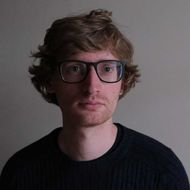
\includegraphics[width=0.95in,height=\textheight]{images/gm.jpeg}

\subcaption{\label{}Г. А. Мороз}
\end{minipage}%
%
\begin{minipage}{0.50\linewidth}

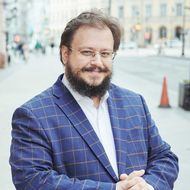
\includegraphics[width=0.95in,height=\textheight]{images/bo.jpeg}

\subcaption{\label{}Б. В. Орехов}
\end{minipage}%

\end{figure}%

\begin{itemize}
\tightlist
\item
  (Санкт-Петербург) Лаборатория языковой конвергенции
\end{itemize}

\begin{figure}

\begin{minipage}{0.50\linewidth}

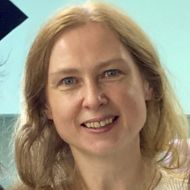
\includegraphics[width=0.95in,height=\textheight]{images/tsh.jpg}

\subcaption{\label{}Т. Ю. Шерстинова}
\end{minipage}%
%
\begin{minipage}{0.50\linewidth}

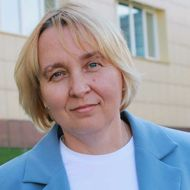
\includegraphics[width=0.95in,height=\textheight]{images/ak.jpeg}

\subcaption{\label{}А. В. Колмогорова}
\end{minipage}%

\end{figure}%
\end{frame}

\begin{frame}{О проекте}
\phantomsection\label{ux43e-ux43fux440ux43eux435ux43aux442ux435-1}
Актуальность проекта состоит в применении к большим текстовым массивам
современных средств обработки естественного языка. Применения методов
компьютерной лингвистики становится опытным полигоном для выявления
границ и возможностей группы компьютерных методов в исследовании языка и
текста.
\end{frame}

\begin{frame}{Подпроекты (Москва):}
\phantomsection\label{ux43fux43eux434ux43fux440ux43eux435ux43aux442ux44b-ux43cux43eux441ux43aux432ux430}
\begin{itemize}
\tightlist
\item
  Построение ландшафта лингвистики на основе аннотаций
\item
  Культуронимическое исследование
\item
  Тематическое моделирование на корпусе текстов «Прожито»
\item
  Создание языковых моделей для решения задач computational literary
  studies
\end{itemize}
\end{frame}

\begin{frame}{Подпроекты (Санкт-Петербург):}
\phantomsection\label{ux43fux43eux434ux43fux440ux43eux435ux43aux442ux44b-ux441ux430ux43dux43aux442-ux43fux435ux442ux435ux440ux431ux443ux440ux433}
\begin{itemize}
\tightlist
\item
  Моделирование картин мира писателя и поколения посредством
  компьютерного анализа больших коллекций художественных текстов
  (корпуса русского рассказа, корпуса текстов личной библиотеки
  С.Довлатова и его собственных сочинений, корпуса фанфиков)
\item
  Создание устного корпуса речи молодежи и дополнение корпуса русского
  рассказа
\item
  Методология описания ``социального настроения эпохи'' посредством
  компьютерного анализа коллекций текстов, находящихся на периферии
  идеологичности: корпуса открыток, корпуса текстов учебников по истории
  России, корпуса советских песен
\item
  Разработка методов эмоциональной разметки текстов разной жанровой
  природы
\item
  Исследование категории естественности устной и письменной речи в
  контексте задачи автоматической генерации текста
\end{itemize}
\end{frame}

\section{Задачи первого этапа
проекта}\label{ux437ux430ux434ux430ux447ux438-ux43fux435ux440ux432ux43eux433ux43e-ux44dux442ux430ux43fux430-ux43fux440ux43eux435ux43aux442ux430}

\begin{frame}{Построение ландшафта лингвистики: задачи}
\phantomsection\label{ux43fux43eux441ux442ux440ux43eux435ux43dux438ux435-ux43bux430ux43dux434ux448ux430ux444ux442ux430-ux43bux438ux43dux433ux432ux438ux441ux442ux438ux43aux438-ux437ux430ux434ux430ux447ux438}
\begin{itemize}
\tightlist
\item
  определение
\end{itemize}
\end{frame}

\begin{frame}{Культуронимическое исследование: задачи}
\phantomsection\label{ux43aux443ux43bux44cux442ux443ux440ux43eux43dux438ux43cux438ux447ux435ux441ux43aux43eux435-ux438ux441ux441ux43bux435ux434ux43eux432ux430ux43dux438ux435-ux437ux430ux434ux430ux447ux438}
\end{frame}

\begin{frame}{Тематическое моделирование на корпусе текстов «Прожито»:
задачи}
\phantomsection\label{ux442ux435ux43cux430ux442ux438ux447ux435ux441ux43aux43eux435-ux43cux43eux434ux435ux43bux438ux440ux43eux432ux430ux43dux438ux435-ux43dux430-ux43aux43eux440ux43fux443ux441ux435-ux442ux435ux43aux441ux442ux43eux432-ux43fux440ux43eux436ux438ux442ux43e-ux437ux430ux434ux430ux447ux438}
\end{frame}

\begin{frame}{Создание языковых моделей для решения задач computational
literary studies: задачи}
\phantomsection\label{ux441ux43eux437ux434ux430ux43dux438ux435-ux44fux437ux44bux43aux43eux432ux44bux445-ux43cux43eux434ux435ux43bux435ux439-ux434ux43bux44f-ux440ux435ux448ux435ux43dux438ux44f-ux437ux430ux434ux430ux447-computational-literary-studies-ux437ux430ux434ux430ux447ux438}
\end{frame}

\section{Результаты первого этапа
проекта}\label{ux440ux435ux437ux443ux43bux44cux442ux430ux442ux44b-ux43fux435ux440ux432ux43eux433ux43e-ux44dux442ux430ux43fux430-ux43fux440ux43eux435ux43aux442ux430}

\begin{frame}{Доклады}
\phantomsection\label{ux434ux43eux43aux43bux430ux434ux44b}
\begin{itemize}
\tightlist
\item
  \textbf{4 октября}: Международная конференция «Дизайн
  междисциплинарных исследований в контексте сближения моделей
  естественно-научного и гуманитарно-социального знания», МФТИ. Г. А.
  Мороз «Построение ландшафта лингвистики: первые результаты и поиск
  стыков с другими науками»
\item
  \textbf{19 октября}: Международная конференция «Русская и зарубежная
  филология в диалоге культур», Южный федеральный университет. Г. А.
  Мороз «Построение ландшафта лингвистики: первые результаты»
\end{itemize}
\end{frame}

\begin{frame}{Формы взаимодействия с каспусом СПб}
\phantomsection\label{ux444ux43eux440ux43cux44b-ux432ux437ux430ux438ux43cux43eux434ux435ux439ux441ux442ux432ux438ux44f-ux441-ux43aux430ux441ux43fux443ux441ux43eux43c-ux441ux43fux431}
\begin{itemize}
\tightlist
\item
  \textbf{16 июня}: открытый очно-заочный семинар, посвященный открытию
  Лаборатории языковой конвергенции в Санкт-Петербурге и презентации
  междисциплинарного проекта
\item
  \textbf{24 октября}: круглый стол «Естественное мышление vs
  искусственный интеллект через призму исследований больших языковых
  данных»
\item
  \textbf{19--21 октября}: Всероссийская научно-практическая конференция
  «Русская и зарубежная филология в диалоге культур»
\item
  Ведение закрытого и открытого Телеграм-каналов для обсуждения текущих
  вопросов, онлайн и очные встречи (март, июнь, сентябрь, ноябрь,
  декабрь).
\end{itemize}
\end{frame}

\section{Планы продолжения
проекта}\label{ux43fux43bux430ux43dux44b-ux43fux440ux43eux434ux43eux43bux436ux435ux43dux438ux44f-ux43fux440ux43eux435ux43aux442ux430}

\begin{frame}{Планы продолжения проекта}
\phantomsection\label{ux43fux43bux430ux43dux44b-ux43fux440ux43eux434ux43eux43bux436ux435ux43dux438ux44f-ux43fux440ux43eux435ux43aux442ux430-1}
\begin{itemize}
\tightlist
\item
  активно взаимодействовать с коллегами из кампуса СПб
\item
  продолжать исследования в рамках описанных нарпавлений
\item
  подготовить публикации по заявленным направлениям:
\end{itemize}

\begin{longtable}[]{@{}
  >{\raggedright\arraybackslash}p{(\columnwidth - 6\tabcolsep) * \real{0.7973}}
  >{\raggedleft\arraybackslash}p{(\columnwidth - 6\tabcolsep) * \real{0.0676}}
  >{\raggedleft\arraybackslash}p{(\columnwidth - 6\tabcolsep) * \real{0.0676}}
  >{\raggedleft\arraybackslash}p{(\columnwidth - 6\tabcolsep) * \real{0.0676}}@{}}
\toprule\noalign{}
\begin{minipage}[b]{\linewidth}\raggedright
название
\end{minipage} & \begin{minipage}[b]{\linewidth}\raggedleft
2023
\end{minipage} & \begin{minipage}[b]{\linewidth}\raggedleft
2024
\end{minipage} & \begin{minipage}[b]{\linewidth}\raggedleft
2025
\end{minipage} \\
\midrule\noalign{}
\endhead
Публикации в научных журналах, входящих в Список А & 0 & 0 & 1 \\
Публикации в научных журналах, входящих в Список B, C, D & 2 & 2 & 2 \\
Прочие публикации в научных журналах, входящих в ядро РИНЦ & 2 & 2 &
2 \\
Главы в рецензируемых монографиях & 0 & 1 & 0 \\
РИД & 1 & 0 & 1 \\
\bottomrule\noalign{}
\end{longtable}
\end{frame}



\end{document}
